\begin{frame}{La bataille navale}
  \scriptsize
    \begin{columns}
      \column{0.6\textwidth}
        Jouons à la bataille navale avec un.e partenaire.
        Voici les règles:
        \begin{itemize}
          \item Vous aurez 6 bateaux qui prennent les nombres de cases \gloss{squares} suivants:
          \begin{itemize}
            \scriptsize
            \item 2 cases (x2), 3 cases (x2), 4 cases, 5 cases
          \end{itemize}
          \item Mettez vos bateaux où que \gloss{wherever} vous voulez sur le plateau.
          \item Votre partenaire va deviner une case, où se trouve peut-être un de vos bateaux, en construisant une phrase d'un mot de la colonne et un verbe de la ligne.
          \begin{itemize}
            \scriptsize
            \item Par ex., tu + tomber (imp) $\to$ tu tombais
          \end{itemize}
          \item Si c'est une case où vous avez un bateau, marque la case.
          \item Si toutes les cases d'un bateau sont choisies, le bateau est coulé \gloss{sunk}.
          \end{itemize}
      \column{0.4\textwidth}
        \small
        Mots utiles:
        \begin{itemize}
          \item toucher \gloss{to hit}
          \item rater \gloss{to miss}
          \item couler \gloss{to sink}
        \end{itemize}
        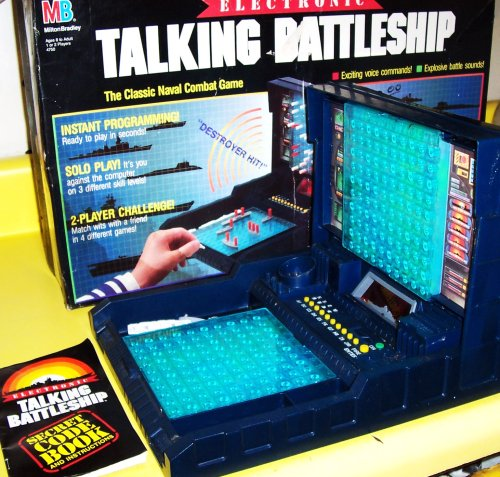
\includegraphics[scale=0.25]{battleship.jpg}
    \end{columns}
\end{frame}